\chapter{Theoretical Background}
\label{cap:Background}

\section{Musical Abilities}
Musical abilities are part of the general musicality of humans. The concept of musicality is a complex and multifaceted phenomenon that has intrigued scholars and researchers across various disciplines for centuries \cite{Gembris1987, Pausch2022, Roman-Caballero2018}. Defining musicality precisely and universally presents several challenges due to its subjective nature, and the interdisciplinary perspectives through which it can be examined.  This chapter aims to highlight some of the difficulties encountered in defining musicality and discusses the issue of developing musical abilities. Additionally, different approaches assessing musical abilities pose their own set of complications and are presented.

\subsection{Definition}
In dictionaries, musicality often refers to a combination of musical abilities, acoomplishments, and  knowledge \cite{MerriamWebster}. The Oxford Enlish Dictionary defines musicality as, "the quality or character of being musical; accomplishment or aptitude in music; musical sensibility" \cite{OED}. This concept points to the usual expected musical skills, like considering them "good" or "skilled" musical knowledge. As a construct, musicality encompasses a wide range of abilities and behaviors that can be categorized into different levels \cite{Gembris1987}. Of these, musical abilities constitute one of the most significant domains within musicality. Defining and structuring musical abilities is a complex task, similar to the challenge of defining (musical) intelligence in general. Researchers have explored various theoretical frameworks and approaches to capture the multifaceted nature of musical abilities.
Two prominent perspectives exist in understanding mucial abilities: the concept of a general musical factor and the identification of specific musical domains.\\
One approach draws parallels between musical abilities and Spearman's general intelligence factor \cite{Spearman1904}. Just as general intelligence is believed to underlie various cognitive abilities, some researchers propose the existence of a general musical factor that influences overall musical aptitude \cite{Mackintosh2011}. This general factor is thought to encompass a range of musical skills, such as pitch discrimination, rhythm perception, tonal memory, and melodic perception. Supporters of this view argue that a common underlying factor contributes to an individual's proficiency across different musical domains \cite{Pausch2022}.
In contrast to the concept of a general musical factor, other scholars emphasize the existence of distinct musical domains. This perspective aligns with Thurstone's theory of primary mental abilities, which suggests that intelligence is composed of multiple specific factors \cite{Thurstone1931}. Similarly, researchers propose that musical abilities can be categorized into separate domains, such as pitch, dynmaic, rhythm, timbre, and tonal memory. Each domain is considered to represent a unique set of skills and competencies within the broader realm of musical abilities. This domain-specific view recognizes the diversity and complexity of musical talents and acknowledges that individuals may excel in certain domains while exhibiting average or lower proficiency in others. This approach underlies Gardner's theory of multiple intelligences, which posits that human intelligence is comprised of distinct modalities, including musical intelligence \cite{Gardner2006}. According to Gardner, musical intelligence involves sensitivity to rhythm, pitch, melody, and timbre, as well as the ability to express oneself musically and appreciate different musical forms. This theory suggests that musical abilities are not confined to a single factor, but rather encompass a range of skills and talents.
While the debate between a general musical factor and domain-specific abilities continues, it is important to recognize that musical abilities are multifaceted and can manifest differently in individuals. Some individuals may demonstrate exceptional proficiency in one or more musical domains while showing average or below-average performance in others. Furthermore, cultural and environmental factors can shape the development of musical abilities, leading to variations across individuals and contexts \cite{Pausch2022}.
In summary, musicality encompasses a range of skills, attributes, and sensitivities that go beyond musical performance alone. It includes the ability to perceive, interpret, express, create, collaborate, and critically analyze music. Musicality enriches our engagement with music, whether as performers, composers, improvisers, active listeners, or music enthusiasts, and it plays a vital role in the human experience of this art form. Overall, understanding musical abilities requires a nuanced approach that acknowledges the potential existence of a general musical factor, the presence of specific musical domains, and the influence of cultural and environmental factors. Future research in this field can further contribute to our understanding of the underlying mechanisms and interactions that shape musical aptitude and performance.




\subsection{Measuring Musical Abilities}
\label{cap:musicalabilities}
\minisec{Musicality tests}
There are various approaches and methods used to assess and test musicality, each focusing on different aspects of musical abilities and skills. It is suggested that musical abilities can be measured through different tests that assess various domains of musical abilities \cite{Werner2016}. In addition to assessing performance, which is the most obvious observation when testing musical abilities, aural skill tests can be employed \cite{Harrison2018, MacGregor2019, Harrison2017}. These tests measure an individual's ability to perceive and recognize musical elements, such as pitch, rhythm, melody, and harmony, through listening exercises. Tasks such as melodic dictation, rhythmic dictation, interval recognition, chord identification, and harmonic analysis are often included in aural skills assessments. They evaluate a person's auditory perception, memory, and understanding of music. 
Tests related to musical perception and analysis assess an individual's ability to analyze and interpret musical compositions \cite{Lee2020}. They can involve listening to musical excerpts and answering questions about the structure, style, form, tonality, and expressive elements present in the music. Assessors evaluate critical listening skills and the ability to articulate musical observations. 
Musical aptitude tests aim to assess a person's innate musical abilities and potential \cite{Gordon1968}. These tests explore various dimensions of musicality, including pitch discrimination, rhythm perception, tonal memory, and melodic perception. Musical aptitude tests provide insights into a person's predisposition towards musical activities and learning. 
Some assessments incorporate psychological and cognitive measures to evaluate musicality. These tests may explore factors such as musical intelligence, working memory, attention, executive functions, and emotional responses to music \cite{Mullensiefen2013}. Psychological and cognitive assessments provide a broader understanding of the cognitive and emotional processes underlying musical abilities.
As explained before there are also supporters who speak of one general musicality factor. For that Wing \cite{Wing1961} developed a "Standardized Test of Musical Intelligence" which measures different skills that supposidly form a whole musical factor. On the other hand Seashore \cite{Seashore1919} developed a "Measure of Musical Talent" which computes a mulitfactorial apporoach of relativley independent musical abilities. 
It is important to note that no single test can fully capture the complexity and diversity of musicality. Therefore, a comprehensive assessment of musicality often involves a combination of these approaches, considering multiple facets of musical abilities, skills, knowledge, and experiences.

\minisec{Assessing Musical Performance}
Rating musical performance is a complex task that requieres a delicate balance between objective assessment and subjective interpretation. To explore musical performances several computer-based algorithms for audio analysis are developed \cite{Goebl2014}. As they have shown usable for detecting timing, amplitude and pitch in musical performances, there are still many limitations and technical challenges. Since musical performances involve subjective qualitites, they are challenging for computer algorithms to capture accurately. With human raters who bring own expertise and experience, small nuances and artistic intent can be examined with which algorithms may struggle to comprehend. Especially adapting to beginner performances, which often have mistakes and lack fluency in their playing is challenging for computer algorithms since they are designes to work with established patterns and data. The ability of human raters to appreciate the subjective, expressive, and contextutal elements of music, adapt to different styles and skill levels, and provide nuanced evaluation offers them distinct advantages over computer-based algorithms in assessing musical performance. Still, when assessing musical performance many aspects have to be taken into count. 

McPhearson and Thompson \cite{McPhearson1998} provided a comprehensive summary of the literature regarding the assessment of musical performance, which is depicted in Figure \ref{fig:assess}. To assess "musical performance", various other domains must be considered. Factors such as the "performance context" (e.g., type, purpose, and proportions of the performance) and the "purpose of assessment" (e.g., ranking in competition or research) already influence the evaluation of musical performance. Several musical and non-musical factors can impact the assessment of musical performance. Musical factors, including the choice of repertoire, ensemble size, and expressivity in accordance with the specific composer or period, can affect the rating of a musical performance. Research has demonstrated that non-musical factors, such as the order of appearance, can influence the evaluation of different musical performances \cite{Flores1996}. Listening to various performances of the same piece may result in a greater appreciation of the composition or cause evaluators to begin with higher expectations that gradually adjust to the reality of the performance. Consequently, the characteristics of both the performer and the evaluator are crucial in assessing musical performance. If the performer experiences anxiety or difficulty concentrating during the performance, it significantly impacts the overall quality. Similarly, the personality of the evaluator also plays a significant role. Although research has indicated that training in adjudication does not guarantee better or more consistent evaluation results \cite{Fiske1977}, the evaluator's mood, attitude, and emotional state can influence their assessments. Furthermore, individual listeners' preferences and subjective experiences play a crucial role in the evaluation of musical performance. Musical tastes and preferences vary widely, and what resonates with one listener may not have the same impact on another.  Additionally, the familiarity between the evaluator and performer can substantially impact the evaluation provided. The selection of evaluative criteria is probably the most complex factor for assessing musical performance. To maximise the reliability within the ratings of the evaluators providing a standardised rating scales has proven useful. They establish criteria and guidelines that can be applied uniformly across different performances and context. This constistency allows more reliable comparisons and assessments, enabling performers to track their progress over time. For constructing such scale different criteria are suggested. As first contributor Duerksen provided eight criteria, including rhythmic accuracy, pitch accuracy, tempo, accent, dynamics, tone quality, interpretation, and overall quality \cite{Duerksen1972}. This foundational framework has paved the way for subsequent research. Russell's study devided evaluation criteria into two categories: technical and musical. Technical aspets encompassed tone, intonation, rhythmic accuracy, articulation, and technique, ehile the musical realm involved tempo, dynamics, timbre, interpretaion, and musical expression. Notably, the component of expression had a significant direct effect on the overall perception of quality \cite{Russell2010}. Within institutional frameworkds, the Australian Music Examination Board's Piano syllabus for level 1 underscores accuracy, fluency, rhythmic and metric stability, articulation, dynamics, phrasing, tonal balance, tempo control, and understanding of style and character \cite{AMEB}. The Associated Board of the Royal Schools of Music marking criteria emphasize pitch, time (fluency and rhythm), tone (articulation and dynamics), shape (expressiveness), and overall performance \cite{ABRSM}. Despite the breadth of research and diverse perspectives on performance criteria, a consensus has shown. For evaluation piano beginners' performance the focus lies on technical aspects such as tone and rhythmic accuracy, fluency, articulation, and dynamics, while expressivity complements the components to an overall performance evaulation. \\
In conclusion, the objective rating of musical performance is a complex tast due to the subjectivity of music, the multidimensionality of its elements, the influence of interpretation and artistic choices, contextual considerations, the interplay between technical accuracy and expressive qualities, listener variability, and the limitations of quantitative metrics. While objective measures can provide some insights, a complete evaluation necessitates a balanced approach that incorporates subjective assessments, export judgment, listener feedback, and an appreciation for the artistic an emotional dimensions that make music a captivating and deeply personal form of expression.

\begin{figure}[]
	\centering
	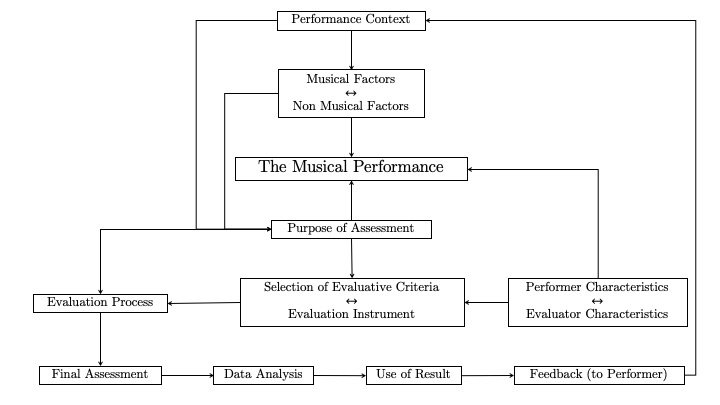
\includegraphics[width=15cm,height=10cm,keepaspectratio]{Assessing}
	\caption{Process Model of Assessing Musical Performance (adapted from \cite{McPhearson1998}))}
	\label{fig:assess}
\end{figure}
\subsection{Development of Musical Abilities}

%### 1. Introduction: stages of musical development, factors influencing musical aptitude, and strategies for nurturing musical skills.
%
%### 2. Stages of Musical Development
Research into the development of musical abilities is mulitfaceted. This includes investigations into infants' perception of structured sound patterns, exploring the connections between learning language and music, and analyzing the context of childrens' musical activities \cite{Forrester2015}. The studies mainly adopted a longitudinal methodological approach studying the same children over a specific time period. 
%### 3. Factors Influencing Musical Aptitude
%- Genetic Predisposition:
%- Explain how genetics can play a role in musical talent, citing studies on heritability and musicality.
%- Environmental Influences:
%- Discuss the impact of early exposure to music, family support, and cultural background on musical development.
%- Neurological Factors:
%- Explore the connection between musical abilities and brain structure, including the role of neuroplasticity.
%- Motivation and Practice:
%- Emphasize the importance of deliberate practice and intrinsic motivation in honing musical skills.
%
%### 4. Nurturing Musical Skills
%- Early Childhood Interventions:
%- Provide recommendations for parents and caregivers to engage young children in musical activities that foster development.
%- Formal Music Education:
%- Discuss the benefits of formal music lessons, including instrument training, singing, and music theory.
%- Informal Learning:
%- Explore the role of self-directed learning, online resources, and peer collaboration in developing musical abilities.
%- Cross-Disciplinary Approaches:
%- Highlight how skills from other domains (mathematics, language) can complement musical development.
%
%### 5. Challenges and Strategies
%- Address common challenges individuals might face during musical development, such as frustration or plateaus.
%- Offer strategies for overcoming these challenges, including setting goals, seeking mentorship, and experimenting with new styles.
%
%### 6. Case Studies and Examples
%- Include real-life examples of individuals who have developed exceptional musical abilities and describe their journeys.
%
%### 7. Conclusion
%- Summarize the key points discussed in the chapter.
%- Emphasize the lifelong nature of musical development and the importance of continued exploration and growth.


The musical development is part of the individual development (ontogenose) \cite{Gembris1987} and can therefore be discussed following the principles of the general psychology of development.


Was bedeutet "Musik lernen"? Hier: ein Musikinstrument lernen\\

welche Parameter befähigen zum Erlernen welcher musiklaischer Fähigkeiten?

Russell \cite{Russell2010} devides skills in technical and musical aspects.  \\\\



%Musical abilities are developed through a combination of innate talent, exposure to music, deliberate practice, and educational opportunities. Here are some key factors that contribute to the development of musical abilities:
%
%1. Early Exposure to Music: Exposure to music from an early age, whether through listening to music, singing, or playing simple instruments, can foster a foundation for musical development. Early exposure helps individuals develop a sense of pitch, rhythm, and musical patterns, laying the groundwork for further musical growth.
%
%2. Natural Aptitude and Talent: Some individuals possess inherent musical abilities and talents, such as an exceptional ear for pitch, rhythmic sensitivity, or an innate sense of musical expression. While talent alone is not sufficient for musical development, it can provide a head start and facilitate progress in specific musical areas.
%
%3. Musical Training and Education: Formal music training, such as private lessons, group classes, or participation in school or community music programs, plays a crucial role in developing musical abilities. Quality instruction and structured learning help individuals acquire technical skills, music theory knowledge, and performance techniques. Music educators provide guidance, feedback, and personalized instruction to nurture musical growth.
%
%4. Deliberate Practice: Deliberate practice refers to purposeful and focused practice aimed at improving specific musical skills. It involves breaking down complex musical tasks into smaller components, setting goals, and engaging in repetitive practice with targeted feedback and adjustments. Regular and disciplined practice sessions help refine technical proficiency, accuracy, expressiveness, and overall musicality.
%
%5. Performance Opportunities: Engaging in regular performance opportunities, such as recitals, concerts, competitions, or informal jam sessions, is vital for developing musical abilities. Performing in front of an audience helps build confidence, stage presence, and the ability to communicate and express oneself through music. It also provides valuable feedback and motivates further improvement.
%
%6. Diverse Musical Experiences: Exploring and experiencing a wide range of musical genres, styles, and traditions contributes to musical development. Exposure to diverse musical cultures and genres enhances musical understanding, creativity, and adaptability. It broadens one's musical palette and encourages the exploration of different techniques, expressions, and interpretations.
%
%7. Active Listening: Actively listening to a variety of music with focused attention and curiosity is essential for musical development. Active listening involves analyzing musical structures, identifying different elements, and discerning the nuances and intentions of the music. This practice enhances musical perception, interpretation, and appreciation.
%
%8. Collaboration and Ensemble Playing: Engaging in ensemble playing, whether in a band, orchestra, choir, or other musical groups, fosters important skills such as listening, teamwork, communication, and synchronization. Collaborative experiences provide opportunities to develop musicality in a social context, supporting the development of sensitivity, adaptability, and musical expression within a group setting.
%
%9. Lifelong Learning and Exploration: Musical abilities continue to develop and evolve throughout a person's lifetime. A commitment to ongoing learning, exploring new musical experiences, and seeking inspiration from diverse sources are essential for continuous musical growth. This involves attending concerts, studying different musical traditions, experimenting with new instruments or genres, and staying open to new musical influences and ideas.
%
%It's important to note that the development of musical abilities is a unique and individual journey. The rate and extent of development can vary among individuals based on factors such as motivation, dedication, access to resources, and personal circumstances.
%
%\section{Music Training and Cognition}
%\label{cap:cognition}
%Music training has long been recognized for its numerous benefits, not only in terms of musical proficiency but also in the impact on the brain and  cognitive processes.This chapter aims to explore the intricate relationship between music, the brain, and cognition, shedding light on the various ways in which music affects our cognitive abilities. By examining empirical studies and theoretical frameworks, this chapter aims to shed light on the potential cognitive benefits of music training and their implications for enhancing overall cognitive functioning.
%
%\minisec{Music Training and Executive Functions}
%Executive functions refer to a set of higher-order cognitive processes that are essential for goal-directed behavior, decision-making, and self-regulation. These functions include working memory, cognitive flexibility, inhibitory control, attentional control, and problem-solving. Music training has been proposed as a potential avenue for enhancing executive functions due to the cognitive demands and complexity involved in learning and performing music. This section explores the relationship between music training and executive functions, highlighting the evidence supporting the cognitive benefits of music education.
%
%Several studies have investigated the impact of music training on various aspects of executive functions. Music training requires individuals to engage in activities that demand sustained attention, working memory, and the ability to integrate multiple sensory and motor processes. As a result, musicians often exhibit enhanced executive function skills compared to non-musicians.
%
%Working memory, the cognitive system responsible for temporarily holding and manipulating information, has been found to be positively influenced by music training. Musicians demonstrate superior performance on working memory tasks, such as digit span, n-back tasks, and complex span tasks. The practice of playing and memorizing music pieces requires musicians to maintain and manipulate musical information in real-time, thus promoting the development and capacity of their working memory.
%
%Cognitive flexibility, the ability to switch between different mental sets or tasks, is another executive function that benefits from music training. Musicians often engage in improvisation and sight-reading, which demand quick adaptation and switching between different musical styles, rhythms, and harmonies. This exposure to diverse musical experiences fosters cognitive flexibility by training individuals to be adaptable and flexible in their thinking.
%
%Inhibitory control, the ability to suppress irrelevant or impulsive responses, is also enhanced through music training. Musicians need to exercise control over their playing technique, timing, and dynamics, requiring them to inhibit automatic or prepotent responses. This practice of inhibitory control in music performance can generalize to other domains of life, leading to improved inhibitory control in non-musical contexts.
%
%Attentional control, the ability to regulate and sustain attention, is another executive function influenced by music training. Musicians exhibit enhanced attentional control, which can be attributed to the demands of reading sheet music, coordinating multiple musical parts, and attending to different musical elements simultaneously. Music training improves individuals' ability to maintain focus, ignore distractions, and allocate attention effectively.
%
%Problem-solving skills, which involve the application of cognitive processes to overcome obstacles and find solutions, may also benefit from music training. Learning music involves problem-solving in various aspects, such as understanding musical notation, deciphering complex rhythms, and interpreting musical structures. These problem-solving experiences contribute to the development of analytical thinking and problem-solving abilities.
%
%Neuroscientific studies provide insights into the neural mechanisms underlying the relationship between music training and executive functions. Music training has been associated with structural and functional changes in brain regions involved in executive functions, including the prefrontal cortex, parietal cortex, and basal ganglia. These changes reflect the brain's adaptive response to the demands of music practice and support the development of enhanced executive function skills.
%
%In conclusion, music training has been linked to improvements in executive functions such as working memory, cognitive flexibility, inhibitory control, attentional control, and problem-solving. The cognitive demands of music practice and performance contribute to the development and enhancement of these executive function skills. By incorporating music training into educational and therapeutic programs, it is possible to harness the potential of music education to promote and strengthen executive functions in individuals of all ages.
%
%References: (Please note that the references are not included here due to the model's response limitations. However, you can find relevant research articles and resources by conducting a literature search using keywords related to this section of the chapter, such as "music training," "executive functions," "working memory," "cognitive flexibility," and "neuroscientific studies.")
%
%\minisec{Cogntive Flexibility and Music Training}
%Cognitive flexibility refers to the ability to adapt one's thinking and switch between different mental processes or strategies in response to changing situations or tasks. It plays a crucial role in problem-solving, creativity, and effective decision-making. Music training has been suggested as a potential facilitator of cognitive flexibility, providing individuals with opportunities to engage in complex and flexible thinking. This section explores the relationship between music training and cognitive flexibility, examining the evidence supporting the notion that music education can enhance this cognitive skill.
%
%Studies investigating the impact of music training on cognitive flexibility have yielded promising results. For instance, research has shown that musicians, compared to non-musicians, exhibit superior performance on tasks that require mental flexibility and the ability to switch between different cognitive sets. This advantage is attributed to the inherent demands of musical training, which often involves reading sheet music, improvisation, and playing different musical pieces with varying styles and structures.
%
%The processes involved in music performance, such as sight-reading, require musicians to constantly adapt and adjust their playing techniques based on the musical notation and the expressive intent of the composition. These demands likely contribute to the development of cognitive flexibility, as musicians learn to quickly switch between different musical elements, interpret complex musical patterns, and respond dynamically to musical cues.
%
%Moreover, music training encourages individuals to explore different musical genres, styles, and techniques, expanding their musical repertoire. This exposure to diverse musical experiences can foster cognitive flexibility by broadening individuals' perspectives and encouraging them to embrace different ways of thinking and expressing themselves musically.
%
%Neuroscientific studies provide further insights into the neural mechanisms underlying the relationship between music training and cognitive flexibility. Functional magnetic resonance imaging (fMRI) studies have revealed that musicians exhibit enhanced connectivity and communication between brain regions involved in cognitive flexibility, such as the prefrontal cortex and the parietal cortex. These findings suggest that long-term engagement in music training can promote structural and functional changes in the brain, supporting the development of cognitive flexibility.
%
%Although the majority of research focuses on the effects of music training on cognitive flexibility in musicians, some studies have also explored the potential benefits of music interventions in non-musical populations. These studies have demonstrated that short-term music training or exposure to music-based interventions can lead to improvements in cognitive flexibility measures, suggesting that even a brief engagement with music activities can have a positive impact on this cognitive skill.
%
%In conclusion, music training has been associated with enhanced cognitive flexibility. The complex and adaptive nature of music performance, coupled with exposure to diverse musical experiences, may contribute to the development of flexible thinking abilities. Furthermore, neuroscientific evidence supports the idea that music training promotes structural and functional changes in the brain, facilitating cognitive flexibility. By recognizing the potential of music education in fostering cognitive flexibility, educators and researchers can explore innovative ways to integrate music training into educational settings and promote the development of this vital cognitive skill.
%
%\minisec{Transfer Effects and Generalization}
%
%One of the intriguing aspects of music training is its potential to generate transfer effects, which refer to the application and generalization of skills and cognitive benefits from music training to other domains of cognition and everyday life. This section explores the concept of transfer effects and generalization in the context of music training, examining the evidence supporting the idea that the cognitive benefits gained through music education can extend beyond the realm of music itself.
%
%Research suggests that music training can lead to transfer effects and generalization to various cognitive domains. For example, the cognitive skills developed through music training, such as working memory, attention, and cognitive flexibility, have been found to benefit academic achievement in areas such as mathematics and language skills. Music training may enhance the ability to manipulate and process information, leading to improved problem-solving and reasoning skills that can be applied in different contexts.
%
%Transfer effects have been observed in the domain of language, where individuals with music training tend to exhibit enhanced phonological awareness, vocabulary skills, and reading abilities. Music training involves attending to the nuances of pitch, rhythm, and timbre, which may contribute to the development of auditory discrimination skills and phonological processing abilities. These skills, in turn, support language acquisition and reading comprehension.
%
%Moreover, transfer effects of music training have been reported in the realm of motor skills. Learning to play a musical instrument involves fine motor control, coordination, and precision. These motor skills developed through music training can transfer to other motor tasks, such as handwriting, sports, and activities requiring manual dexterity.
%
%Neuroscientific research provides insights into the neural mechanisms that underlie transfer effects and generalization from music training. Music training has been associated with changes in brain structure and function, including increased connectivity between brain regions involved in cognitive processes. These neural changes may enhance the efficiency and flexibility of information processing, allowing individuals to apply skills learned in the context of music to other cognitive tasks and domains.
%
%It is important to note that transfer effects may vary across individuals and depend on factors such as the duration and intensity of music training, the age at which training begins, and the specificity of the transfer task. The extent of transfer may also be influenced by the similarity between the cognitive processes engaged during music training and the target domain. For example, transfer effects from music training to language skills may be stronger due to the overlap in auditory processing and phonological awareness.
%
%Overall, while transfer effects and generalization from music training are evident, they are not universal and may vary depending on multiple factors. Nonetheless, the potential for transfer highlights the value of music education as a holistic approach to cognitive development. By engaging in music training, individuals can acquire cognitive skills that can be applied across various domains, promoting lifelong learning and enhancing overall cognitive abilities.
%
%References: (Please note that the references are not included here due to the model's response limitations. However, you can find relevant research articles and resources by conducting a literature search using keywords related to this section of the chapter, such as "music training," "transfer effects," "generalization," and "neural mechanisms.")
%
%
%
%
%
%\minisec{Music Training and Neuroplasticity}
%Neuroplasticity refers to the brain's ability to reorganize and adapt its structure and function in response to experiences, learning, and environmental changes. It plays a fundamental role in shaping cognitive abilities and is a key mechanism underlying the cognitive benefits of music training. This section explores the relationship between music training and neuroplasticity, highlighting how engaging in music education can lead to structural and functional changes in the brain.
%
%Numerous studies have provided compelling evidence for the neuroplastic effects of music training. Long-term engagement in music practice has been associated with structural changes in brain regions involved in auditory processing, motor control, and executive functions. For instance, studies have shown that musicians have increased gray matter volume in areas such as the auditory cortex, motor cortex, prefrontal cortex, and corpus callosum compared to non-musicians. These structural changes reflect the fine-tuning of neural circuits that support musical skills and the integration of sensory, motor, and cognitive processes.
%
%Functional neuroimaging techniques, such as functional magnetic resonance imaging (fMRI) and electroencephalography (EEG), have provided insights into the functional changes that occur in the brains of musicians. Research has shown that music training can enhance the activation and connectivity between brain regions involved in auditory processing, memory, attention, and executive functions. Musicians often demonstrate heightened activation in the auditory cortex, suggesting increased sensitivity to sound and improved auditory processing. Moreover, musicians exhibit enhanced connectivity between brain regions within the frontotemporal network, which is crucial for various cognitive functions.
%
%The effects of music training on neuroplasticity are not limited to musicians. Short-term music interventions and even passive exposure to music have been shown to induce temporary changes in brain activity and connectivity. For instance, listening to music has been found to modulate neural responses, including the release of neurotransmitters associated with reward and emotional processing. These temporary changes in brain activity demonstrate the immediate influence of music on neural processes and provide a basis for further exploration of music-based interventions.
%
%The timing and intensity of music training appear to be important factors influencing neuroplastic changes. Long-term, intense music training, starting at an early age, tends to have more pronounced effects on brain structure and function. However, even modest engagement with music training can lead to measurable changes in the brain. Additionally, the specific components of music training, such as playing an instrument or singing, may result in differential patterns of neuroplasticity.
%
%The implications of neuroplasticity extend beyond the cognitive benefits of music training. Understanding the brain's capacity to change and adapt has important implications for rehabilitation and interventions targeting cognitive and motor impairments. Music-based interventions have shown promise in neurorehabilitation, aiding individuals with stroke, Parkinson's disease, and other neurological conditions in regaining motor skills, improving speech, and enhancing cognitive functions.
%
%In conclusion, music training is associated with neuroplastic changes in the brain. Long-term engagement in music practice can lead to structural and functional adaptations, reflecting the brain's capacity to reorganize in response to musical experiences. These neuroplastic changes contribute to the cognitive benefits observed in musicians and highlight the potential of music-based interventions for promoting brain health and rehabilitation. Further research is needed to explore the specific mechanisms and long-term effects of music training on neuroplasticity.
%

\section{Aging}
The aging process exerts profound effects on diverse cognitive domains, including learning abilities. While it is commonly believed that learning becomes more challenging with age, research indicates that older adults are still capable of acquiring new knowledge and skills, albeit with some differences and considerations. Understanding the relationship between aging and learning is crucial for promoting lifelong learning and maintaining cognitive vitality in older individuals. Given the impact of music on the brain, as discussed in Chapter \ref{cap:cognition}, exploring its impact on aging adds an intriguing dimension to the investigation 


\subsection{Music and Aging}

%Musical Engagement in aging
The impact of music on brain functions, especially in the context of healthy elderly individuals, has been a subject of increasing interest in recent years. This section explores how musical engagement affects cognitive, emotional, and physical well-being in older adults, highlighting the transformative power of music and its potential to enhance the qualitiy of life during the aging process.

%significance of musical engagement during aging
Music holds the capacity to evoke emotions and enhance subjective well-being in older adults \cite{Croom2015}. Familiar and personally meaningful music music can trigger nostalgia, evoke positive memories, and create a sense of emotional connectedness \cite{?}. Music therapy interventions have been found to reduce anxiety, depression, and stress, contributinf to emotional well-being in older adults \cite{Guetin2013}. These emotional benefits contribute to an overall improvement in the psychological state of older individuals \cite{?}. Especially piano training has demonstrated the ability to enhance psychosocial outcomes in older adults over a three-month period \cite{Bugos2022}.

%positive effects on physical health and functionality
Engaging in musical activities can have positive effects on physical health and functional abilities in older adults. Playing a musical instrument, singing, and participating in dance or rhythmic movement can improve motor coordination, balance, gait, and overall physical fitness \cite{?}. Musical interventions, such as rhythmic auditory stimulation, have been used to enhance motor rehabilitation in individuals with age-related mobility impairments \cite{Thaut2015}. In the realm of stroke motor rehabilitation, music-based interventions show promise due to their tool integration of motor training and multimodal stimulation \cite{Grau-Sanchez2020}. 

%Catalyst for social interaction and connection
Furthermore, music serves as a powerful catalyst for social interaction and connection among older adults. Group music-making activities provide opportunities for social engagement, fostering a sense of belonging and community. The implementation of music-based interventions in senior living communities or nursing homes encourages social interaction, reduces feelings of isolation, and improves overall social well-being \cite{Creech2013}.

%Profound effects on cognitive functions
Numerous studies have shown the impact of music on various cognitive functions in older adults. The concept of far transfer effect indicates a connection between musical training and improvements in executive function, attention, working memory, verbal and visual memory, and sensorimotor function \cite{Bugos2007, Dege2018, Hanna-Pladdy2011}. 
These cognitive benefits can be attributed to the multisensory stimulation, complex auditory processing, and motor coordination required during musical activities, particularly musical instrumental practice \cite{Seinfeld2013}. The engagement in lifelong musical practice has been found to confer cognitive advantages compared to individuals without musical experience, as evidenced by older musicians displaying greater gray matter volume and white matter advantages compared to those without musical experience \cite{James2014}. Furthermore, engagement in musical activities has been associated with a reduced risk of age-related cognitive decline and dementia \cite{Balbag2014}. This preventive effect extends to both recent and past musical activities, which have shown to delay cognitive decline and dementia \cite{Hanna-Pladdy2011, Hanna-Pladdy2012}. Music therapy has also been shown to effectivly restore motor skills post-stroke \cite{Grau-Sanchez2020, Altenmuller2020}. Overall, music training holds promise as an approach to mitigate age-related cognitive decline and promote healthy aging \cite{Klimova2017}.

%sustaining youthful brain function
A recent study suggests that music may even sustain youthful brain function \cite{Rogenmoser2018}. A comparison of chronological age and  "brain age" among amateur musicians, musicians, and non-musicians revealed that amateur musician exhibit the lowest scores, suggesting an age-decelerating effect of musicon the brain. However, subsequent studies have not replicated these findings \cite{Matziorinis2023}. It is proposed that musical training and active musical engagement may be linked to the challenge resilience factor, potentially contributing to a form of neurocognitive reserve.

In summary, the impact of music engagement on older adults is substantial, encompassing emotional well-being, physical health, cognitive function, and social interaction. By understanding these effects, we can appreciate the potential for structured musical instruction to significantly impact the lives of aging individuals. While the majority of research focuses on the effects of music training on cognitive aging, it is important to note that individual differences and factors such as the duration and intensity of training can influence outcomes. Additionally, the specific components of music training, such as instrumental practice or singing, may have differential effects on cognitive aging.



\subsection{Learning and Aging}

Aging is associated with certain cognitive changes that can impact learning. These changes include a decline in the executive functions, such as processing speed, working memory capacity, inhibition, cognitive flexibility and fluid intelligence \cite{Grady2012, Reuter-Lorenz2010}. 

%Lifelong Learning's Significance in Aging

%%The concept of lifelong learning underscores the continuous process of acquiring knowledge and skills throughout life. This section introduces the importance of ongoing learning in maintaining cognitive vitality and adaptive thinking in older adults.
Contrary to earlier beliefs, research has shown that the adult brain retains a remarkable degree of neuroplasticity, even in old age \cite{Altenmuller2020}. Neuroplasticity refers to the brain's ability to reorganize and form new neural connections. This means that the aging brain remains capable of adapting and rewiring in response to learning experiences. Engaging in learning activities has numerous benefits for older adults, including cognitive stimulation, social engagement, and personal growth. 
The concept of lifelong learning refers to the continuous pursuit of knowledge and skills throughout one's life \cite{Leipold2012}. Lifelong learning is thought of ongoing cognitive stimulation, which is essential for maintaining cogntive function and preventing cognitive decline and can take various forms, such as formal education, vocational training, hobbies, and self-directed learning. Engaging in new learning experiences challenges the brain, promotes neural plasticity, and help preserve memory, attention, and other cogntive abilities \cite{?}. Learning new skills and acquiring knowledge in later life fosters adaptive thinking and problem-solving abilities. It enables older adults to approach novel challenges with a flexible mindset and develop effective strategies for navigating various situations \cite{?}. 


%The Role of Lifelong Learning in Cognitive Reserve

%%Exploring the notion of cognitive reserve, this sub-section delves into how engaging in learning activities across the lifespan contributes to cognitive resilience and a potential buffer against cognitive decline in aging.

Cognitive reserve is a concept rooted in neuroscience and psychology, describing the brain's capability to optimize performance through two mechanisms: the recruitment of brain networks and compensation using alternative cognitive strategies \cite{Nucci2012}. The essence of cognitive reserve lies in the brain's proactive response to damage by using pre-existing cognitive processes or enlisting compensatory strategies. This implies that people with a high cognitive reserve can withstand more age-related changes and disease-related pathologies by effectively using cognitive paradigms or alternative brain networks \cite{Stern2009}. Studies indicate that reserve is correlated with better cognitive performance in adulthood \cite{Panico2022}. 
Cogntive reserve is influenced by education, occupational activities and leisure pursuits \cite{Nucci2012}. Years of formal education and possible training courses contribute to cognitive reserve. Working activities also plays a predictive ole for better cognitive reserve, where the degrees of intellectual involvement and personal responisbility, coupled with the duration of engagement, is important. The quality and quantity of engaging in cognitive stimulating leisure activities, such as reading, playing music, and participating in social and physical pursuits, further can impact cognitive reserve.
The underlying mechanisms behind cognitive reserve are not yet fully understood, but researchers believe that it involves greater neuronal connectivity, the ability to recruit alternative brain networks, and a more efficient use of brain resources when performing cognitive tasks.
It's important to note that cognitive reserve doesn't provide absolute protection against cognitive decline or brain diseases, but it can delay the onset of symptoms or reduce the severity of cognitive impairment. Encouraging activities that promote cognitive reserve throughout life can be beneficial in maintaining brain health and improving the quality of life as we age.

% Cognitive Flexibility: Adapting to New Challenges
	% Cognitive Flexibility's Relevance in Aging
	%%This section highlights the significance of cognitive flexibility—an essential cognitive skill—in addressing novel challenges and adapting to changing circumstances during the aging process.
Cognitive flexibility, a fundamental cognitive skill in acquiring new abilities, underscores the capacity to switch between thinking about two different concepts or to consider multiple concepts simultaneously \cite{Scott1962}. This cognitive aptitude holds a central role in various cognitive processes demanding shifts in attention and adaptability. Greater cognitive flexibility is associated with better quality of life in older adults \cite{Davis2010}. The adaptability resulting within cognitive flexibility is necessary in adressing new challenges, adapting to changing circumstances, and learning new skills during the aging process. The intricate interplay of cognitive flexibility with salience detenction, attention, inhibition, working memory, and switching underscores its significance \cite{Dajani2015}.


	%Nurturing Cognitive Flexibility through Lifelong Learning
	%%Building upon the previous subsection, this part emphasizes how continuous learning fosters cognitive flexibility, making the connection between adaptive learning experiences and enhanced cognitive agility.


% Learning Challenges in Aging: Strategies for Success
	%Learning Challenges Associated with Aging
	%%Delving into the cognitive changes associated with aging, this section explores how factors like processing speed and working memory may impact learning efficiency.
	
The overall decrease in working memory capacity may explain the deterioration of executive functions \cite{Zinke2014}. In aging brains, both global connectivity (the networks of long-range cortical fiver structural connections, known as white matter) and functional connectivity (the information flow dynamics throughout the whole brains) have been found to be less efficient \cite{Spreng2013}. Cognitive regression is associated with local structural and functional brain modifications, including reduction of gray matter in the prefrontal cortex and hippocampus, and loss of anterior white matter integrity and functional connectivity. The hippocampus plays a crucial role in various forms of relational memory, and atrophy in this area can lead to deterioration in working and long-term memory, as well as a drecrease in abstract thinking. This decline in cognitive abilities increases the risk for dementia. However, engaging in cognitive abilities and physical exercise can potentially delay age-related atrophy in the hippocamus or even expand its size \cite{Erickson2011, Fotuhi2012}. 
As the brain functions change, not all cognitive functions decline with age. Crystallized intelligence, which refers to accumulated knowledge and expertise, tends to remain stable or even improve over time \cite{Stemmler2013}. Additionally, older adults may adopt compensatory strategies and rely more on their existing knowledge and experiences to facilitate learning. The developmental trajectory during aging is influenced by a combination of physiological and cognitive functions, with the potential for ongoing growth through leraning and interventions.

	%Overcoming Learning Challenges: Effective Strategies
	%%Presenting strategies to overcome learning challenges, this subsection discusses methods such as breaking down complex tasks, consistent practice, and creating a supportive learning environment.

Older adults may face specific challenges when engaging in learning activities \cite{Zeki2021}. For example, age-related changes in sensory perception, such as hearing and vision impairments, can affect the acquisition of new information. Furthermore, older adults may experience increased cognitive load and require additional time to process and integrate new information. However, these challenges can be mitigated through appropriate instructional design, tailored learning approaches, and the use of assistive technologies.

To counteract cognitive decline, different therapy approaches have been developed. Therapies that rely on everyday activities such as dancing, musical training, or playing chess have been shown to induce a far-reaching transfer of learning due to their variabolity and complexitiy \cite{Shawn2008, Shawn2014}. It is important to progressivly increase the difficulty of learning activities to maintain challenge and intrinsic motivating. Several studies have demonstrated brain changes in aging adults. For instance, three months of learning how to juggle increased gray matter volume in the left hippocampus of 60-year-olds without significant differences compared to younger participants \cite{Boyke2008}. Aerobic training induced volume increases in the prefrontal cortex, anterior hippocampus and white matter integrity after 12 months \cite{Hedden2004, Erickson2011, Colcombe2006}. Musical practice has been found to induce funtional and structural plasticity in the anterior and middle part of the hippocampus, resulting in increased profiency in musical tasks, improved working memory, and enhanced fluid intelligence \cite{Oechslin2013, Groussard2010, Herdener2010, James2008}. Learning to read mucial notation over three months induced special effects on visuo-spatial skills und on the fusiform gyrus und superior parietal areas in initially muscially naïve adults \cite{Stewart2003, Stewart2005}. Five weeks of musical training for adult novices led to functional audio-motor coupling in the temporal-frontal regions, indicating brain plasticity \cite{Lappe2008, Bangert2003, Lahav2007}. Piano practice over 4-6 Monate enhanced executive functions and working memory \cite{Seinfeld2013, Bugos2007}. Drumming and singing improved verbal and visual memory \cite{Dege2018}. Generally, learning a new skill engages neural plasticity more strongly in older adults \cite{Greenwood2010}. 


%The Role of Motivation and Personalization
	%Motivation's Impact on Learning in Aging
	%%Exploring the importance of motivation, this section emphasizes how an intrinsic desire to learn plays a pivotal role in sustaining engagement and achievement in learning activities.

%Personalized Learning: Tailoring to Individual Needs
	%%This sub-section introduces the concept of personalized learning, explaining how adapting instruction to individual preferences enhances motivation and optimizes the learning process for older adults.


%Setting the Stage for Musical Learning and Development
	%The Intersection of Learning Principles and Music
	%%Building upon the groundwork laid in previous subsections, this part establishes a bridge between the discussed learning concepts and the upcoming focus on musical learning and development.

	%Musical Learning as a Vehicle for Lifelong Learning
	%%Concluding this subchapter, this section introduces the idea that musical learning embodies the principles of continuous learning, cognitive flexibility, and motivational factors discussed earlier, making it an ideal avenue for enhancing cognitive well-being and adaptive skills in aging individuals.




In summary, although there are age-related changes in cognition, older adults are still capable of learning and acquiring new knowledge and skills. By understanding the challenges and implementing effective strategies, lifelong learning can be promoted, providing cognitive stimulation, personal growth, and social engagement for older individuals. Embracing a proactive approach to learning can contribute to maintaining cognitive vitality and overall well-being throughout the aging process.




durch musizieren cognitive flexibilty erhalten?

%Lifelong learning and skill acquisition
	%	Examine the concept of lifelong learning and its application to acquiring new skills, including musical abilities, in older adults.
	%	Discuss the potential benefits of engaging in skill-based activities like learning a musical instrument.
	%	Highlight the importance of tailored instruction and motivation in promoting successful skill acquisition.
%Musical Learning and Aging
	%	Review research on the capacity of older adults to learn and develop new musical abilities.
	%	Discuss studies that emphasize the adaptability of aging brains to musical training and skill refinement.
	%	Address the potential challenges and advantages associated with learning music later in life.
%2.4 Assessing Musical Abilities in Elderly Adults
	%Present methods and tools for assessing musical abilities, including performance skills, auditory perception, rhythm comprehension, and music theory understanding.
	%Discuss the relevance of adapting assessment strategies to accommodate the unique needs and experiences of elderly learners.
	%Highlight the importance of considering both qualitative and quantitative measures in evaluating musical progress.
%2.5 The Role of Structured Instruction and Longitudinal Studies
	%Explain the significance of structured instruction in developing musical abilities among elderly adults.
	%Discuss the benefits of using longitudinal study designs to observe the progression of musical skills over time.
	%Address potential challenges and ethical considerations in conducting long-term studies with older participants.
%2.6 Conceptual Framework: Enhancing Musical Abilities through Structured Instruction
	%Develop a conceptual framework that illustrates the interaction between structured musical instruction and the development of musical abilities.
	%Highlight the potential pathways through which focused learning can lead to improved musical proficiency.
	%Emphasize the role of motivation, practice, and individualized instruction in promoting sustained musical engagement.
 
 
 


\section{Aims/Hypothesis}
musical instrumental prcatice can countervail cognitive and perceptual-motor decline supported by functional and structural brain plasiticity ==> naja, ist nicht mein approach
\\promote healthy mental aging in elderly - independence, autonomy and well-being through musical activities